% Title: glps_renderer figure
% Creator: GL2PS 1.3.8, (C) 1999-2012 C. Geuzaine
% For: Octave
% CreationDate: Mon May 22 01:44:38 2017
\setlength{\unitlength}{1pt}
\begin{picture}(0,0)
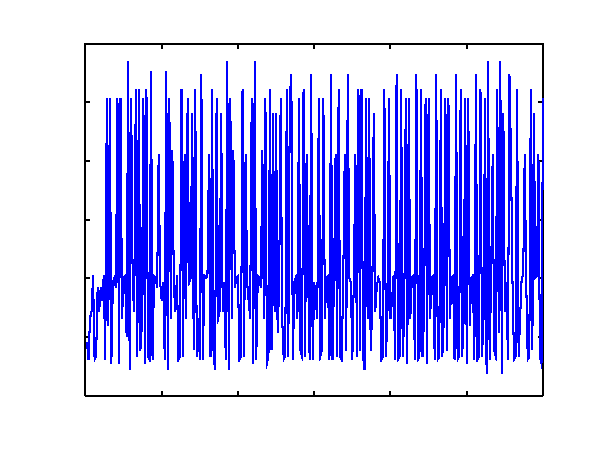
\includegraphics{q12-inc}
\end{picture}%
\begin{picture}(288,218)(0,0)
\fontsize{10}{0}
\selectfont\put(41.0044,22.9956){\makebox(0,0)[t]{\textcolor[rgb]{0,0,0}{{0}}}}
\fontsize{10}{0}
\selectfont\put(77.6104,22.9956){\makebox(0,0)[t]{\textcolor[rgb]{0,0,0}{{50}}}}
\fontsize{10}{0}
\selectfont\put(114.216,22.9956){\makebox(0,0)[t]{\textcolor[rgb]{0,0,0}{{100}}}}
\fontsize{10}{0}
\selectfont\put(150.822,22.9956){\makebox(0,0)[t]{\textcolor[rgb]{0,0,0}{{150}}}}
\fontsize{10}{0}
\selectfont\put(187.428,22.9956){\makebox(0,0)[t]{\textcolor[rgb]{0,0,0}{{200}}}}
\fontsize{10}{0}
\selectfont\put(224.034,22.9956){\makebox(0,0)[t]{\textcolor[rgb]{0,0,0}{{250}}}}
\fontsize{10}{0}
\selectfont\put(260.64,22.9956){\makebox(0,0)[t]{\textcolor[rgb]{0,0,0}{{300}}}}
\fontsize{10}{0}
\selectfont\put(36.0127,27.9961){\makebox(0,0)[r]{\textcolor[rgb]{0,0,0}{{0.2}}}}
\fontsize{10}{0}
\selectfont\put(36.0127,56.1631){\makebox(0,0)[r]{\textcolor[rgb]{0,0,0}{{0.3}}}}
\fontsize{10}{0}
\selectfont\put(36.0127,84.3306){\makebox(0,0)[r]{\textcolor[rgb]{0,0,0}{{0.4}}}}
\fontsize{10}{0}
\selectfont\put(36.0127,112.498){\makebox(0,0)[r]{\textcolor[rgb]{0,0,0}{{0.5}}}}
\fontsize{10}{0}
\selectfont\put(36.0127,140.666){\makebox(0,0)[r]{\textcolor[rgb]{0,0,0}{{0.6}}}}
\fontsize{10}{0}
\selectfont\put(36.0127,168.833){\makebox(0,0)[r]{\textcolor[rgb]{0,0,0}{{0.7}}}}
\fontsize{10}{0}
\selectfont\put(36.0127,197){\makebox(0,0)[r]{\textcolor[rgb]{0,0,0}{{0.8}}}}
\fontsize{10}{0}
\selectfont\put(150.822,11.9956){\makebox(0,0)[t]{\textcolor[rgb]{0,0,0}{{t}}}}
\fontsize{10}{0}
\selectfont\put(17.0127,112.498){\rotatebox{90}{\makebox(0,0)[b]{\textcolor[rgb]{0,0,0}{{$E_{out}(g_t)$}}}}}
\fontsize{10}{0}
\selectfont\put(150.822,207){\makebox(0,0)[b]{\textcolor[rgb]{0,0,0}{{Result of Question 12}}}}
\end{picture}
